% JASA template — Permutations Accelerate Approximate Bayesian Computation
% TEST
\PassOptionsToPackage{unicode}{hyperref}
\PassOptionsToPackage{hyphens}{url}
\PassOptionsToPackage{dvipsnames,svgnames,x11names}{xcolor}

\documentclass[12pt]{article}

%%% ---- Packages ----
\usepackage[]{natbib}
\bibliographystyle{agsm}

\usepackage[english]{babel}
\usepackage{amsmath}
\usepackage{amssymb}
\usepackage{amsthm}
\newtheorem{theorem}{Theorem}[section]
\newtheorem{lemma}[theorem]{Lemma}
\newtheorem{corollary}[theorem]{Corollary}
\newtheorem{proposition}[theorem]{Proposition}
\theoremstyle{remark}
\newtheorem{remark}[theorem]{Remark}
\theoremstyle{plain}

\usepackage{lmodern}
\usepackage{bm}
\usepackage{bbold}
\usepackage{graphicx}
\usepackage{subcaption}

\usepackage{tikz}
\usetikzlibrary{matrix,fit,backgrounds,positioning}
\usepackage{pgfplots}
\pgfplotsset{compat=1.18}

\usepackage[ruled,noend]{algorithm2e}
\usepackage{xcolor}
\usepackage[normalem]{ulem}

\DeclareMathOperator*{\argmax}{arg\,max}
\DeclareMathOperator*{\argmin}{arg\,min}

\makeatletter
\renewcommand{\algocf@captiontext}[2]{#1\algocf@typo. \AlCapFnt{}#2}
\renewcommand{\AlTitleFnt}[1]{#1\unskip}
\def\@algocf@capt@plain{top}
\renewcommand{\algocf@makecaption}[2]{%
  \addtolength{\hsize}{\algomargin}%
  \sbox\@tempboxa{\algocf@captiontext{#1}{#2}}%
  \ifdim\wd\@tempboxa >\hsize
    \hskip .5\algomargin%
    \parbox[t]{\hsize}{\algocf@captiontext{#1}{#2}}%
  \else
    \global\@minipagefalse%
    \hbox to\hsize{\box\@tempboxa}%
  \fi
  \addtolength{\hsize}{-\algomargin}%
}
\makeatother

%%% ---- JASA margins ----
\addtolength{\oddsidemargin}{-.5in}%
\addtolength{\evensidemargin}{-.1in}%
\addtolength{\textwidth}{1in}%
\addtolength{\textheight}{1.7in}%
\addtolength{\topmargin}{-1in}

%%% ---- Hyperref ----
\usepackage{hyperref}
\hypersetup{
  pdftitle={Permutations Accelerate Approximate Bayesian Computation},
  pdfauthor={A. Luciano; C. Andral; C. P. Robert; R. J. Ryder},
  pdfkeywords={Approximate Bayesian Computation, Sequential Monte Carlo,
    Hierarchical models, Permutation-based inference, Likelihood-free methods},
  colorlinks=true,
  linkcolor={blue},
  filecolor={Maroon},
  citecolor={Blue},
  urlcolor={Blue},
}

%%% ---- User macros ----
\input{preamble/defs}

%%% ---- Override: hide \old{} text to test page count ----
\renewcommand{\old}[1]{}

%%% ---- Anonymization toggle ----
% Set \anon to 0 for anonymous version (review), 1 for identified version
\newcommand{\anon}{1}

\date{}

%%% ============================================================
\begin{document}

\def\spacingset#1{\renewcommand{\baselinestretch}%
{#1}\small\normalsize} \spacingset{1}

%%%%%%%%%%%%%%%%%%%%%%%%%%%%%%%%%%%%%%%%%%%%%%%%%%%%%%%%%%%%%%%%%%%%%%%%%%%%%%

\if1\anon
{
  \title{\bf Permutations Accelerate Approximate Bayesian Computation}
  \author{
    A.~Luciano\thanks{
      Antoine Luciano is supported by a PR[AI]RIE PhD grant.},
    C.~Andral, and
    C.~P.~Robert \thanks{
      Christian P. Robert is also affiliated with the University of Warwick, UK and is funded by the European Union under the GA 101071601, through the 2023-2029 ERC Synergy grant OCEAN and by a PR[AI]RIE chair from the Agence Nationale de la Recherche (ANR-19-P3IA-0001).} \\
    CEREMADE, UMR CNRS 7534, Universit\'e Paris Dauphine PSL\\[6pt]
    and \\[6pt]
    R.~J.~Ryder \\
    Department of Mathematics, Imperial College London}
  \maketitle
} \fi

\if0\anon
{
  \bigskip
  \bigskip
  \bigskip
  \begin{center}
    {\LARGE\bf Permutations Accelerate Approximate Bayesian Computation}
  \end{center}
  \medskip
} \fi

\bigskip
\begin{abstract}
\input{sections/abstract}
\end{abstract}

\noindent%
{\it Keywords:}
Sequential Monte Carlo; Hierarchical models;
Permutation-based inference; Likelihood-free methods; Exchangeability
\vfill

\newpage
\spacingset{1.8} % DON'T change the spacing!


%%% ---- Main text ----

\section*{Introduction}
\input{sections/0_intro}

\section{From ABC to permABC}
\label{secabc_to_permabc}

In this section, we will review the ABC framework and highlight its limitations within the hierarchical model framework. Subsequently, we will introduce our permutation-based method, permABC, which aims to address these limitations.

\subsection{Introduction to ABC}


The standard rejection ABC algorithm, often referred to as \emph{Vanilla ABC}, proceeds by drawing parameters from the prior distribution, $\param \sim \pi(\cdot)$, and then simulating synthetic data from the likelihood, $\simdata \sim f(\cdot \mid \param)$. The pair $(\param, \simdata)$ is accepted if the summary statistics of the simulated data are sufficiently close to those of the observed data, that is, if $d(\eta(\obsdata), \eta(\simdata)) \leq \varepsilon$ for some tolerance level $\varepsilon > 0$ and some summary statistic $\eta$. This procedure yields samples from the approximate joint distribution $\pi_{\varepsilon}\{\param,\simdata \mid \eta(\obsdata)\}$; we marginalize out $\simdata$ to get the ABC posterior

\begin{equation}
    \label{eqabc}
    \begin{split}
        \pi_{\varepsilon}(\param \mid \eta(\obsdata)) &\propto
        \int_{\dataspace^\Clust} \pi_{\varepsilon}(\param, \simdata \mid \eta(\obsdata)) \, d\simdata \\
        &\propto \pi(\param) \int_{A_{\obsdata,\varepsilon}} f(\simdata \mid \param) \, d\simdata,
    \end{split}
\end{equation}
where $A_{\obsdata,\varepsilon} = \{\simdata \in \dataspace^\Clust \mid d(\eta(\obsdata), \eta(\simdata)) \leq \varepsilon\}$ denotes the acceptance region.

Combining an informative summary statistic $\eta$ with a small tolerance $\varepsilon$ typically leads to a good approximation of the true posterior distribution, so that $\pi_{\varepsilon}(\param \mid \eta(\obsdata)) \approx \pi(\param \mid \obsdata)$. This approximate posterior—often called a \emph{pseudo-posterior}—is obtained by replacing the true likelihood $f(\obsdata \mid \param)$ with the integral of the likelihood over the neighborhood $A_{\obsdata,\varepsilon}$ of the observed data, effectively using it as a surrogate for the intractable likelihood.

Throughout this work, we assume for clarity that the data are compared directly, i.e., $\eta = \mathrm{Id}$. Under this assumption, the acceptance region simplifies to the $\varepsilon$-ball $B_{\varepsilon}(\obsdata)$ centered at $\obsdata$ with respect to the distance $d$. Nonetheless, the proposed method naturally extends to the use of low-dimensional summary statistics.


In our numerical examples, we take $\dataspace = \mathbb R^n$ and use the distance $d(\cdot,\cdot)$ between two datasets in \( \dataspace^K \), each consisting of \( K \times n \) observations, defined as follows: 
\begin{equation}
    \label{eqdistance}
    d(\obsdata, \simdata) = \sqrt{\sum_{k=1}^K w_k^2 \| \obsdata_k - \simdata_k \|_2^2},
\end{equation}
where \( \| \cdot \|_2 \) denotes the Euclidean norm, and the weights \( w_k \) are used to control the relative influence of each compartment in the distance computation. The weight vector \( w_{1:K} \) can either be manually specified by the user or selected adaptively to prevent any single compartment from dominating the distance, as suggested by \citet{prangle2017adapting}.


This naive ABC algorithm faces several limitations, including poor scalability in the parameter space and an exponentially increasing computational cost due to the declining acceptance rate as \( \varepsilon \) decreases. In the context of the hierarchical model of Figure \ref{fig:hier}, the acceptance rate further diminishes as the number of compartments \( K \) increases. Simulating a dataset \( \simdata \) from the prior predictive distribution that matches all compartments of \( \obsdata \) within a small tolerance \( \varepsilon \) can be particularly challenging. 


\subsection{Motivations of permABC}

A common approach in ABC to increase the acceptance rate is to exploit the exchangeability of the compartments through a permutation-invariant summary statistic, such as the sorted vector. For instance, when there is a one-dimensional observation (or statistic) per compartment, $\obsdata \in \mathbb{R}^K$, it is natural to use the ordering $\eta(\obsdata)=\mathrm{sort}(\obsdata)$ as a summary. This replaces the $K!$ possible labelings by a canonical representation, thereby simplifying the comparison between datasets.

Moreover, in the univariate case, sorting is known to minimize the distance over all permutations of the simulated data. Specifically, \(
d\bigl(\mathrm{sort}(\obsdata),\mathrm{sort}(\simdata)\bigr)
=
\min_{\sigma\in\mathcal{S}_K} d(\obsdata,\simdata_\sigma),
\)
where $\mathcal{S}_K$ denotes the set of all permutations of $\{1,\dots,K\}$. Equivalently, in this one-dimensional setting, comparing sorted vectors amounts to computing the Wasserstein distance between the empirical measures of the compartments, which connects our construction to Wasserstein ABC (WABC) \citep{bernton2019approximate}.

However, this equivalence should not obscure an important difference in inferential target. WABC is designed to compare samples viewed as unordered point clouds, and is therefore primarily suited to settings where inference concerns global features of the data distribution. By contrast, our setting is hierarchical: inference concerns not only the global parameter \( \globparam \), but also the local parameters \( \locparam_{1:K} \), at least up to relabelling. In particular, WABC is not designed for hierarchical models with compartment-specific local parameters, since it does not keep track of which simulated compartment is associated with which local parameter.

In higher dimension, the scalar sorting argument no longer applies. When each $\obsdata_k$ is a vector in $\mathbb{R}^n$ with $n>1$, there is no canonical ordering that is both deterministic and permutation-optimal. We therefore solve the matching problem directly, which leads to the acceptance criterion
\begin{equation}
    \label{eqopti}
    \min_{\sigma \in \mathcal{S}_K} d(\obsdata,\simdata_\sigma)\le \varepsilon.
\end{equation}

This condition means that the simulated dataset is accepted whenever it matches the observed dataset up to a permutation of the compartments. It can therefore yield a substantial increase in acceptance probability, heuristically of order $K!$ when $\varepsilon$ is small and the neighborhoods associated with distinct permutations are essentially disjoint. The optimization problem in \eqref{eqopti} can be formulated as a linear sum assignment problem, or equivalently a bipartite matching problem, and solved efficiently using a modified Jonker--Volgenant algorithm \citep{jonker1987shortest}, with computational complexity $\mathcal{O}(K^3)$ \citep{crouseImplementing2DRectangular2016a}. Although this remains substantial, it reduces the combinatorial cost from $K!$ to polynomial time and makes problems with up to $K=100$ compartments tractable in practice; see the real-data application in Section~\ref{sec:sir}.

This matching criterion is closely related to optimal transport between the empirical distributions of the compartments. In the multivariate case, \citet{bernton2019approximate} discuss several cheaper approximations to exact transport, including Hilbert-curve sorting, swap-based refinements, and entropically regularized Sinkhorn divergences. These approximations are particularly attractive when the number of points is very large. In our applications, however, $K$ remains only moderately large, while the dimension of each compartment-level observation may be non-negligible. In this regime, solving the assignment problem exactly remains practical and robust. We nevertheless return to this point in Section~\ref{sec:sequential}, where we show that within an SMC scheme a cheaper swap-based refinement, warm-started from the previous iteration's optimal permutation, is sufficient in practice.

However, using \eqref{eqopti} does not yield samples from the pseudo-posterior defined in \eqref{eqabc}, but rather from the following permutation-invariant version:
\begin{equation}
    \label{eqpermabc_tilde}
    \begin{split}
        \Tilde \pi_{\varepsilon} (\param \mid \obsdata)
        &\propto \int_{\dataspace^K} \Tilde \pi_{\varepsilon} (\param,\simdata \mid \obsdata)\, d\simdata \\
        &\propto \pi(\param)\int_{\Tilde A_{\obsdata,\varepsilon}} f(\simdata \mid \param)\, d\simdata,
    \end{split}
\end{equation}
where the acceptance region is
\[
\tilde{A}_{\obsdata,\varepsilon}
=
\left\{
\simdata\in\dataspace^K \;\middle|\;
\min_{\sigma\in\mathcal{S}_K} d(\obsdata,\simdata_\sigma)\le \varepsilon
\right\}
=
\bigcup_{\sigma\in\mathcal{S}_K} B_\varepsilon(\obsdata_\sigma),
\]
with \(B_\varepsilon(\obsdata_\sigma)\) denoting the $\varepsilon$-ball centered at \(\obsdata_\sigma\) for the distance \(d\).

In this formulation, the likelihood \(f(\obsdata\mid\param)\) is approximated by its integral over a neighborhood of all permutations of the observed dataset:
\[
\int_{\tilde A_{\obsdata,\varepsilon}} f(\simdata\mid\param)\, d\simdata
\approx
\sum_{\sigma\in\mathcal{S}_K} f(\obsdata_\sigma\mid\param).
\]

Inference under \eqref{eqpermabc_tilde} is therefore naturally defined only up to a permutation of the local components \( \locparam_{1:K} \), as in WABC \citep{bernton2019approximate}, effectively yielding posterior samples of the form \(
\Tilde{\param}
=
(\globparam,\{\locparam_1,\dots,\locparam_K\}),
\)
where the local parameters are treated as an unordered set. This target may be appropriate when the local parameters are nuisance quantities, but in many hierarchical applications one wishes to recover inference on the ordered local components as well.

To our knowledge, this specific permutation-based formulation of ABC for hierarchical models with local parameters has not been formally studied in the literature. We therefore introduce \emph{permABC}, which exploits permutation matching to improve acceptance while making it possible to recover inference on the full parameter vector \( \param \), including the ordered local parameters.

\subsection{The permABC algorithm}
\label{secpermabc_star}


Restoring identifiability among compartments is essential for enabling inference on the full parameter vector. One natural way to achieve this is by applying a suitable permutation to the accepted parameters, such that the simulated data are optimally aligned with the observed dataset. However, explicitly testing all \( K! \) permutations is computationally intractable.

Fortunately, whenever the acceptance condition \eqref{eqopti} is satisfied, there exists at least one permutation of the simulated dataset that meets the ABC criterion, namely the optimal one minimizing the distance. This permutation, denoted by \( \sigma^* = \argmin_{\sigma \in \mathcal{S}_K} d(\obsdata, \simdata_{\sigma}) \), provides a natural way to reorder the parameter vector.

In practice, the \emph{permABC} algorithm proceeds similarly to standard ABC: we sample \( \parprop \sim \pi(\cdot) \) and simulate data \( \simdata \sim f(\cdot \mid \parprop) \). If the minimum distance over all permutations satisfies the tolerance condition, we accept and return the pair \( (\parprop_{\sigma^*}, \simdata_{\sigma^*}) \). This induces a new pseudo-posterior distribution, denoted \( \pi_{\varepsilon}^*(\cdot, \cdot \mid \obsdata) \), which corresponds to the pushforward of the distribution \( \tilde{\pi}_\varepsilon \) defined in \eqref{eqpermabc_tilde} under the optimal alignment map \( \proj \):

\begin{equation}
\label{eqproj}
\pi^{*}_{\varepsilon}(\cdot, \cdot \mid \obsdata)
:= \projsharp \tilde{\pi}_{\varepsilon}(\cdot, \cdot \mid \obsdata)
\end{equation}
where
\[
\proj: (\param, \simdata) \mapsto (\param_{\sigma^*}, \simdata_{\sigma^*}).
\]
By construction, \( \proj \circ \proj = \proj \), so \( \proj \) acts as a projection. Moreover, its preimage satisfies \( \proj^{-1}(\{\param, \simdata\}) = \{(\param_{\sigma}, \simdata_{\sigma}) \mid \sigma \in \mathcal{S}_K\} \).

As a result, the projected pseudo-posterior satisfies:
\begin{equation*}
    \begin{split}
        \pi_{\varepsilon}^* (\param, \simdata \mid \obsdata) &  \propto \Tilde \pi_{\varepsilon} (\proj^{-1}(\{(\param, \simdata)\}) \mid \obsdata)\cdot \mathbb I_{\text{Im}(\proj)}(\param,\simdata)\\
        & \propto \sum_{\sigma} \Tilde \pi_{\varepsilon} (\param_{\sigma}, \simdata_{\sigma} \mid \obsdata)\cdot \mathbb I_{\text{Im}(\proj)}(\param,\simdata)\\
        % & \propto \sum_{\sigma} \pi(\param_{\sigma}) f(\simdata_{\sigma} \mid \param_{\sigma}) \mathbb{I}_{\tilde A_{\obsdata,\varepsilon}}(\simdata_{\sigma})\cdot \mathbb I_{\text{Im}(\proj)}(\param,\simdata)\\
        % & \propto \pi(\param) f(\simdata \mid \param) \mathbb{I}_{\tilde A_{\obsdata,\varepsilon}}(\simdata)\cdot \mathbb I_{\text{Im}(\proj)}(\param,\simdata)\\
        & \propto \tilde \pi_{\varepsilon}(\param, \simdata\mid \obsdata) \cdot \mathbb I_{\text{Im}(\proj)}(\param,\simdata).
    \end{split}
\end{equation*}


\noindent \old{which enforces a constraint that accepted samples must lie in the image of the projection, i.e., must be optimally aligned with the observed data.

This additional constraint effectively restricts the integration domain to a subset of datasets that are optimally ordered with respect to \( \obsdata \). We define this constrained space as}\new{This restricts accepted samples to the image of \( \proj \). We define the constrained space as}
\[
\dataspace_{\obsdata}^{*K} = \left\{ \simdata \in \dataspace^K \mid d(\obsdata, \simdata) = \min_{\sigma \in \mathcal{S}_K} d(\obsdata, \simdata_{\sigma}) \right\}.
\]
Consequently, the marginal pseudo-posterior can be expressed as:
\begin{equation}
\label{eqpermabc_star}
\pi_{\varepsilon}^*(\param \mid \obsdata) \propto \pi(\param) \int_{A_{\obsdata,\varepsilon}^*} f(\simdata \mid \param) \, d\simdata,
\end{equation}
where the new acceptance region is 
\[
A_{\obsdata,\varepsilon}^* = B_{\varepsilon}(\obsdata) \cap \dataspace_{\obsdata}^{*K}.
\]

The \emph{permABC} algorithm (see Algorithm~\ref{alg:permABC_star}) therefore defines a different approximation of the posterior distribution than classical ABC methods. In particular, it yields a different posterior approximation  \( \pi_{\varepsilon}^*(\cdot \mid \obsdata) \), which we shall compare to the vanilla ABC approximation \( \pi_{\varepsilon}(\cdot \mid \obsdata) \).


\begin{algorithm}
{\small
\SetKwInOut{Inputt}{Input}
\SetKwInOut{Outputt}{Output}
\caption{permABC Vanilla}\label{alg:permABC_star}
\textbf{Input: }observed dataset $\obsdata$, number of iterations $N$, threshold $\varepsilon>0$.\\
\textbf{Output: }a sample $(\param^{(1)}, \dots, \param^{(N)})$ from the pseudo-posterior distribution $\pi_{\varepsilon}^*(\cdot\mid \obsdata)$.\\

\BlankLine

\For{$i = 1,\dots, N$}{
    \Repeat{$d(\obsdata, \simdata_{\sigma^*}) \leq \eps$}{
        $\parprop \sim \pi(\cdot)$\;
        $\simdata \sim f(\cdot \mid \parprop)$\;
        $\sigma^* = \argmin_{\sigma \in \mathcal{S}_K} d(\obsdata, \simdata_{\sigma})$\;
    }
    $\param^{(i)} = \param'_{\sigma^*}\;$
}
}% end \small
\end{algorithm}

\subsection{Comparison with ABC and asymptotic perspective}
\label{sec:comparison}

The permutation step in permABC has two distinct asymptotic interpretations, depending on whether one focuses on the global parameter \(\globparam\) or on the labelled local parameters \(\locparam_{1:K}\).

For the global parameter \(\globparam\), once the labels of the local components are ignored, the acceptance rule of permABC falls within the same Wasserstein-type paradigm as WABC \citep{bernton2019approximate}. In our hierarchical setting, the number of compartments \(K\) plays the role of the sample size in WABC, since the comparison is performed through the empirical distributions of the observed and simulated compartments. This viewpoint is useful because it allows us to directly invoke the asymptotic intuition developed for WABC: when \(\varepsilon \to 0\) with the observations kept fixed, the pseudo-posterior approaches the exact posterior, while as the sample size increases one obtains posterior concentration under suitable identifiability conditions. In our context, this supports the view that the permutation-invariant marginal pseudo-posterior in \(\globparam\) inherits the same qualitative behaviour as \(K\) increases. Moreover, when \(\varepsilon\) is kept fixed, the resulting target should be interpreted as a coarsened posterior rather than as a Dirac mass, in the spirit of \citet{miller2019robust}. 

For the labelled local parameters \(\locparam_{1:K}\), however, the relevant comparison is no longer with WABC but with standard ABC. Indeed, permABC differs from standard ABC in one key aspect: instead of retaining all permutations that satisfy the ABC criterion, it keeps only the optimal one, namely the permutation that minimizes the discrepancy defined in Equation~\eqref{eqopti}. This choice is computationally attractive, but it alters the pseudo-posterior by constraining the pseudo-data to lie in \(\dataspace^{*K}_{\obsdata}\). A stratified variant recovering the standard pseudo-posterior is described in Appendix~\ref{sec:appendix_strat}. We now show that, for small enough \(\varepsilon\), this difference vanishes.

\begin{lemma}
\label{lempermABC_star}
Let \(\obsdata \in \dataspace^K\) denote the observed dataset, and define
\[
\varepsilon^* := \frac{1}{2}\min_{\sigma \neq \mathrm{Id}} d(\obsdata,\obsdata_\sigma).
\]
Then, for any \(\varepsilon < \varepsilon^*\) and any simulated dataset \(\simdata \in \mathbb{R}^{K \times n}\), at most one permutation satisfies the ABC criterion:
\[
\mathrm{Card}\left\{\sigma \in \mathcal{S}_K : d(\obsdata,\simdata_\sigma)\le \varepsilon\right\}\le 1.
\]
\end{lemma}

The proofs of the preceding lemma, the following theorem, and the subsequent corollary are deferred to Appendix~\ref{appendix_proofs}.

We assume that no two compartments have exactly the same observed data. This implies that \(\varepsilon^*>0\), and this condition is satisfied almost surely for continuous data. Under this assumption, permABC and standard ABC coincide for sufficiently small \(\varepsilon\), as stated below.

\begin{theorem}
\label{th:permABC_star}
Let \(\pi^*_{\varepsilon}(\cdot\mid\obsdata)\) denote the pseudo-posterior distribution resulting from permABC, and \(\pi_{\varepsilon}(\cdot\mid\obsdata)\) that obtained from standard ABC. Then, for all \(\varepsilon<\varepsilon^*\),
\[
\pi^*_{\varepsilon}(\cdot\mid\obsdata)=\pi_{\varepsilon}(\cdot\mid\obsdata).
\]
\end{theorem}

This equivalence ensures that permABC inherits the same small-tolerance asymptotic behaviour as standard ABC for the full labelled parameter vector. In particular, any consistency result for ABC immediately transfers to permABC in the regime \(\varepsilon\to0\).

\begin{corollary}
\label{col:permabc}
If the pseudo-posterior distribution \(\pi_{\varepsilon}(\cdot\mid\obsdata)\) obtained by standard ABC converges to the true posterior distribution as \(\varepsilon\to0\), then the pseudo-posterior distribution \(\pi^*_{\varepsilon}(\cdot\mid\obsdata)\) obtained by permABC also converges to the true posterior distribution as \(\varepsilon\to0\).
\end{corollary}

Thus, the efficiency gains provided by permABC come at no cost to asymptotic consistency. More generally, beyond mere consistency, one may appeal to the asymptotic theory developed for ABC by \citet{frazier2018asymptotic}, which gives general results on posterior concentration, limiting posterior shape, and asymptotic distributions under suitable regularity, identifiability, and joint \((n,\varepsilon)\)-asymptotics. In the present hierarchical setting, these results apply to permABC in the regime \(\varepsilon<\varepsilon^*\), where permABC and ABC coincide, while the WABC viewpoint described above provides the appropriate asymptotic interpretation for the marginal pseudo-posterior in \(\globparam\).

\section{Sequential strategy with permutations}
\label{sec:sequential}
\input{sections/2_sequential}

\section{Numerical experiments}
\label{sec:numeric}
\subsection{Comparison between ABC and permABC}
\label{sec:abc_vs_permabc}

As discussed in Section~\ref{sec:comparison}, permABC exhibits a different behavior from standard ABC. In particular, two regimes emerge depending on the value of the threshold \( \varepsilon \): when \( \varepsilon > \varepsilon^* \), permABC yields a different approximation of the posterior compared to ABC; whereas when \( \varepsilon \leq \varepsilon^* \), permABC coincides with standard ABC and thus inherits its convergence guarantees.
% \xian{La question étant quelle approximation est préférable ??}

To better illustrate the differences between the two approaches, we consider a simple toy model with no global parameter, defined as follows:
\[
\mu_k \sim \mathcal{U}(-2, 2), \quad \obsdata_k \sim \mathcal{U}(\mu_k - 1, \mu_k + 1), \quad k = 1, \dots, K,
\]
with \( K = 2 \), and a fixed observation \( y = (-1, 1)^\top \). 

Figure~\ref{fig:unif} highlights the two different regimes. When \( \varepsilon > \varepsilon^* \), permABC is concentrated in a region constrained by the order statistics, leading to a pseudo-posterior different from that of standard ABC. However, when the threshold satisfies \( \varepsilon \leq \varepsilon^* \), both methods recover the same pseudo-posterior. In this example, the critical value is \( \varepsilon^* = \sqrt{1/8}/2 \approx 0.177 \).


Note that, even in its vanilla form, permABC offers a significant gain in simulation efficiency. Since it effectively avoids redundant permutations during rejection, it reduces the required number of simulations by a factor of approximately \( K! \). In this simple example with \( K = 2 \), we achieve the same approximation quality (i.e., same \( \varepsilon < \varepsilon^* \)) using only half the number of simulations compared to standard ABC.

\begin{figure}[htbp]
    \centering
    \includegraphics[scale=.5]{fig/fig3_seed_42.pdf}
    \caption{\old{Comparison between standard ABC (left) and permABC (right) on the toy model of Section \ref{sec:abc_vs_permabc} with \( K = 2 \) and observation \( y = (-1, 1)^\top \). Each dot represents a sampled configuration \( \mu = (\mu_1, \mu_2) \), colored by the acceptance threshold used: purple for \( \varepsilon = \infty \), green for \( \varepsilon > \varepsilon^* \), and yellow for \( \varepsilon = \varepsilon^* \). The black cross denotes the observation \( y \), and the dashed box indicates the true posterior. While both methods recover the same posterior when \( \varepsilon < \varepsilon^* \), permABC avoids simulating permutations that are suboptimal at large \( \varepsilon \), resulting in a more concentrated distribution and improved efficiency. The two panels use the same computational budget.}\new{ABC (left) vs.\ permABC (right) on the uniform toy model with \( K = 2 \). Dots are sampled \( (\mu_1, \mu_2) \) at three tolerance levels: \( \varepsilon = \infty \) (purple), \( \varepsilon > \varepsilon^* \) (green), \( \varepsilon = \varepsilon^* \) (yellow). Both methods agree when \( \varepsilon < \varepsilon^* \); permABC is more concentrated and efficient at equal budget.}}
    \label{fig:unif}
\end{figure}
\subsection{Challenges of High-Dimensional ABC: A Gaussian Toy Model}
\label{sec:gaussian_toy}
We now consider a classical hierarchical model commonly used in the Bayesian literature:
\begin{equation*}
    \label{eqgauss}
    \beta \sim \mathrm{IG}(a,b), \quad \mu_k \sim \mathcal{N}(0, s^2), \quad \obsdata_{k} = (y_{1,k}, \dots, y_{n,k}) \overset{\text{i.i.d.}}{\sim} \mathcal{N}(\mu_k, \beta), \quad k = 1, \dots, K.
\end{equation*}
Throughout this section we set \( a = b = 5 \), \( s = 10 \), \( n = 10 \) observations per component, and \( K = 20 \) unless stated otherwise.

This simple yet representative model provides a convenient testbed to compare the various methods discussed in this paper, and to highlight the limitations of standard ABC approaches in high-dimensional settings. All ABC methods involve a fundamental trade-off between the number of simulations \( N \), the tolerance threshold \( \varepsilon \), and the effective number of accepted samples (or the number of unique particles in sequential schemes). A more efficient method achieves a lower value of \( \varepsilon \) for a given simulation budget \( N \) and fixed final sample size.

To enable fair comparison across methods, we adopt a consistent evaluation criterion: for each experiment, we report the value of \( \varepsilon \) achieved when the algorithm yields exactly 1,000 unique particles. In this setting, the number of simulations required to obtain a single unique accepted sample serves as a proxy for the effective sample size (ESS). This pseudo-ESS provides a normalized measure of sampling efficiency, which we use throughout our benchmarks.

\new{A low tolerance \( \varepsilon \), however, is only a proxy for posterior quality: two methods that target different pseudo-posteriors cannot be compared on \( \varepsilon \) alone. To evaluate the quality of the produced approximation directly, we instead report the sliced Wasserstein-2 distance \citep{bonneel2015sliced,nadjahi2020statistical} between the weighted particle cloud and a reference posterior obtained by long MCMC (PyMC) on the Gaussian toy model of Section~\ref{sec:gaussian_toy}. The sliced Wasserstein metric is well suited to this setting: it metrises weak convergence on \( \mathbb{R}^{d} \), admits linear-time Monte Carlo estimators in the ambient dimension, and has been used as a target discrepancy in ABC by \citet{nadjahi2020approximate}. Reporting \( \mathrm{SW}_2 \) assesses whether the permutation-based gains in tolerance translate into genuinely better posterior approximations.}

Rejection-based algorithms such as vanilla ABC, as well as sequential variants like ABC-SMC and ABC-PMC, are known to scale poorly with the dimension of the parameter space, here indexed by the number of groups \( K \). As \( K \) increases, the acceptance rate drops sharply, resulting in a dramatic rise in computational cost. In contrast, the permutation-based acceptance rule introduced in permABC significantly improves the efficiency of both rejection and sequential samplers in high-dimensional regimes. The symmetry structure across local parameters \( \mu_1, \dots, \mu_K \) allows permABC to reduce redundant simulations and produce sharper approximations of the target pseudo-posterior.

\new{Figure~\ref{fig:vanilla_vs_smc} illustrates this phenomenon in terms of the sliced Wasserstein-2 distance to the reference posterior: permutation-based methods reach substantially lower \( \mathrm{SW}_2 \) values than their non-permuted counterparts at equal simulation budget. In particular, for \( K=20 \) and without outliers, permABC-SMC and permABC-Vanilla plateau roughly \(3\)--\(6\)~times closer to the reference than ABC-SMC or ABC-Vanilla. These gains become increasingly pronounced as \( K \) grows, confirming the advantage of permutation-based strategies in hierarchical or exchangeable models.}

\new{A complementary comparison in terms of wall-clock time — rather than simulation count — yields similar conclusions, and is provided in Appendix~\ref{sec:appendix_comparison}.}

\begin{figure}[htbp]
    \centering
    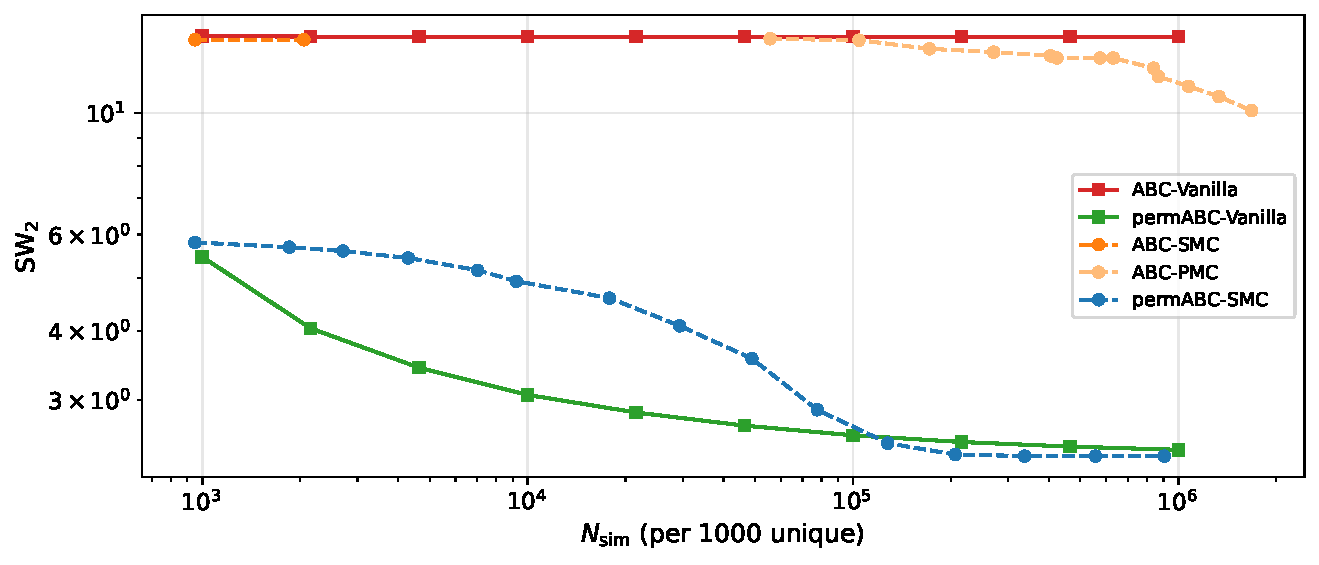
\includegraphics[width=\textwidth]{fig/fig4_sw2_nsim_seed_45.pdf}
    \caption{\new{Sliced Wasserstein-2 distance to the reference posterior vs.\ number of simulations (log--log) for the Gaussian toy model with \( K=20 \), no outliers (\( N_{\mathrm{particles}} = 5{,}000 \)). Permutation-based methods reach substantially lower \( \mathrm{SW}_{2} \) at equal budget. Wall-clock time counterpart in Appendix~\ref{sec:appendix_comparison}.}}
    \label{fig:vanilla_vs_smc}
\end{figure}



\subsection{Failure cases of ABC-Gibbs}
\label{sec:abcgibbs_failure}

ABC-Gibbs methods \citep{clarte2021componentwise,rodrigues2020likelihood} have been designed to handle hierarchical models similar to those we consider. They are however less robust to model dependencies. We illustrate this with a modified hierarchical model designed to highlight the limitations of ABC-Gibbs:
\begin{equation*}
    \label{eqgauss_robin}
    \beta \sim \mathcal{N}(0, 10^2), \quad \mu_k \sim \mathcal{N}(0, 10^2), \quad \obsdata_k = (\obsdata_{1,k}, \dots, \obsdata_{n,k}) \overset{\text{i.i.d.}}{\sim} \mathcal{N}(\mu_k + \beta, 1), \quad k = 1, \dots, K.
\end{equation*}
This model is deliberately over-parameterized: it includes \( K+1 \) parameters for only \( K \) observations. Despite its simplicity, the posterior distribution exhibits a strong ridge structure due to the symmetry between local parameters \( \mu_k \) and the global parameter \( \beta \). This posterior can be reliably approximated using reference MCMC software such as PyMC. 
% \al{closed-form available? — to be computed.}

Figure~\ref{fig:perm_vs_gibbs} shows the two-dimensional marginal posterior over \( (\mu_1, \beta) \) obtained under a fixed simulation budget. While permABC-SMC provides a conservative and coherent approximation of the target posterior—as expected for an ABC method with global proposals—ABC-Gibbs produces a truncated approximation, failing to explore the full posterior support.

\old{This discrepancy is rooted in the very structure of ABC-Gibbs. The algorithm proceeds by sequentially updating each parameter conditionally on the others using ABC rejection steps. In the presence of strong dependencies between parameters, as is the case here, the algorithm exhibits poor mixing: each marginal update is constrained by the current (possibly incorrect) values of the other parameters. As a result, the sampler explores a narrow region of the parameter space, failing to recover the full shape of the posterior.

These results underscore the limitations of coordinate-wise ABC approaches in models with strong local-global coupling. In contrast, permABC-based strategies, which jointly consider the full dataset and parameter configuration at each step, are more robust to such structural challenges.}%
\new{This failure is structural: ABC-Gibbs updates each parameter conditionally on the others, so strong dependencies cause poor mixing. In contrast, permABC jointly considers the full parameter configuration and is robust to such coupling.}




\begin{figure}[htbp]
    \centering
    \includegraphics[scale=.5]{fig/fig5.pdf}
    \caption{\old{Two-dimensional marginal posterior over \( (\mu_1, \beta) \) for the hierarchical model defined in Equation~\eqref{eqgauss_robin}, under a fixed simulation budget. The black ellipses represent level sets of the exact posterior distribution computed via MCMC (PyMC). Blue points correspond to samples produced by permABC-SMC, and red points to those produced by ABC-Gibbs. While permABC-SMC captures the full posterior geometry and respects the strong negative correlation between \( \mu_1 \) and \( \beta \), ABC-Gibbs fails to explore the posterior support. It becomes trapped along a narrow subset of the ridge, leading to a truncated and biased approximation. This illustrates the poor mixing behavior of coordinate-wise ABC samplers in the presence of strong global-local dependencies.}\new{Marginal posterior over \( (\mu_1, \beta) \) for the over-parameterised model~\eqref{eqgauss_robin}. Ellipses: exact MCMC level sets. permABC-SMC (circles) captures the full ridge; ABC-Gibbs (triangles) is trapped in a narrow subset, illustrating poor mixing under strong global--local coupling.}}
    \label{fig:perm_vs_gibbs}
\end{figure}



\subsection{Discussion of the Over-Sampling and Under-Matching Approaches}
\label{sec:osum}

The Over-Sampling and Under-Matching strategies provide two complementary extensions of the permABC framework, each improving robustness and efficiency in different regimes of hierarchical inference under exchangeability.

We evaluate their performance on a Gaussian toy model with \( K = 20 \) compartments, among which 4 have local means \( \mu_k \) lying in the tails of the prior. This setup simulates a realistic scenario involving mild model misspecification or contamination by outliers. \new{Figure~\ref{fig:osum} reports the sliced Wasserstein-2 distance \( \mathrm{SW}_{2} \) between the weighted particle cloud and a reference posterior obtained by long MCMC, as a function of the wall-clock time required to obtain 1{,}000 unique accepted particles. This posterior-quality metric directly measures how close each algorithm gets to the true posterior.}

\new{The Over-Sampling method (permABC-OS) reaches values of \( \mathrm{SW}_{2} \) comparable to standard permABC-SMC at the same runtime, and remains the method of choice in the low-tolerance regime: even though each iteration is more expensive because of larger assignment problems and duplicated particles (see Appendix~\ref{appendix_os}), the additional candidate compartments allow faster progression in the contaminated setting.}

\new{Under-Matching (permABC-UM) is the method that benefits most from the presence of outliers. By relaxing the matching constraint to only \( L<K \) compartments, it allows rapid convergence in \( \mathrm{SW}_{2} \) in the intermediate-tolerance regime while ignoring the worst-matching ones, in line with the behaviour expected from the asymptotic analysis of Section~\ref{sec:permABC_OS}. Empirically, the \( \mathrm{SW}_{2} \) advantage of permABC-UM over permABC-SMC grows almost log-linearly with the number of outliers: on this benchmark, a linear fit on \( \log(\text{ratio}) \) gives a slope of roughly \(-0.12\) to \(-0.16\) per additional outlier for \( K\in\{10,15,20\} \). The same model without contamination does not exhibit such an improvement, confirming that the Under-Matching gain is specifically attributable to outliers. On the other hand, as the algorithm transitions to full matching (\( L_t \to K \)), the acceptance condition tightens and the particle population can degenerate; unlike in the Over-Sampling strategy, this issue cannot be alleviated by duplication, and the method typically fails to reach the lowest \( \mathrm{SW}_{2} \) values.}

These contrasting behaviors suggest that combining the two strategies could yield additional benefits. One possibility is to begin inference with permABC-UM to quickly eliminate poorly fitting regions, then switch to permABC-SMC to refine toward smaller tolerances. More generally, hybrid schemes where \( L_t \) and \( M_t \) are jointly adapted — potentially alternating with changes in \( \varepsilon \) — offer a promising direction for future exploration.

\new{A complementary figure reporting the number of simulations (instead of runtime) is provided in Appendix~\ref{sec:appendix_comparison}.}

\begin{figure}[htbp]
    \centering
    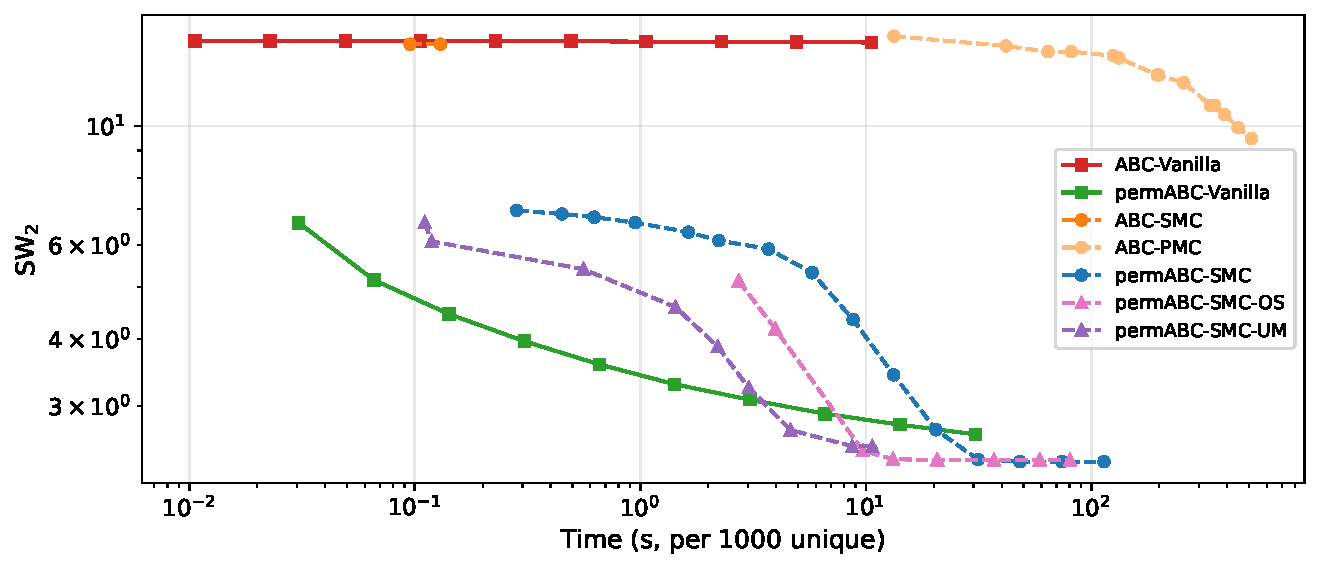
\includegraphics[width=\textwidth]{fig/fig6_sw2_time_seed_45.pdf}
    \caption{\new{\( \mathrm{SW}_{2} \) to reference posterior vs.\ wall-clock time (log--log) for the Gaussian toy model with \( K=20 \) and 4 outliers (\( N_{\mathrm{particles}} = 5{,}000 \)). Under-Matching is most efficient at intermediate tolerances; Over-Sampling remains competitive at low tolerances. Simulation-count counterpart in Appendix~\ref{sec:appendix_comparison}.}}
    \label{fig:osum}
\end{figure}






\subsection{Application to Real Data: The SIR Model}
\label{sec:sir}

In this final section, we illustrate the applicability of our methodology on real-world data by analysing the early spread of COVID-19 in France using publicly available hospitalization records from Santé publique France \citep{DataCovid}. The dataset provides daily hospital admissions at several geographic levels. We focus on mainland France (excluding overseas territories and Corsica), which yields 94 departmental time series.

To describe the epidemic dynamics, we use a classical Susceptible--Infectious--Recovered (SIR) model, defined through the latent system of ordinary differential equations
\begin{equation}
    \label{eqSIR}
    \begin{split}
        \frac{dS}{dt} &= -\delta \frac{SI}{N},\\
        \frac{dI}{dt} &= \delta \frac{SI}{N} - \nu I,\\
        \frac{dR}{dt} &= \nu I,
    \end{split}
\end{equation}
where \(S\), \(I\), and \(R\) denote the numbers of susceptible, infectious, and recovered individuals, respectively, \(N\) is the population size, and \(\delta\) and \(\nu\) are the transmission and recovery rates. The corresponding basic reproduction number is \(R_0 = \delta / \nu\).

\old{Since the available data consist of hospital admissions rather than direct observations of the infectious compartment, the ODE system defines only a latent epidemic trajectory. To obtain simulated datasets, we combine the SIR dynamics with a stochastic observation model. Specifically, the transmission rate at each sub-daily time step is perturbed by a multiplicative log-normal noise:
\[
\delta_k^{(t)} = \delta_k \cdot \exp(\sigma \, \xi_k^{(t)}), \qquad \xi_k^{(t)} \overset{\text{i.i.d.}}{\sim} \mathcal{N}(0,1),
\]
with \(\sigma = 0.05\). This noise captures unmodelled day-to-day variability in transmission---due to reporting delays, local behavioural changes, or stochastic contact patterns---so that the simulated data entering the ABC distance are random even when the underlying SIR dynamics are deterministic. This distinction is important here, as ABC is applied to simulated observations rather than to the deterministic ODE solution itself.}%
\new{Since the data are hospital admissions, the ODE defines a latent trajectory. To introduce stochasticity, the transmission rate is perturbed at each sub-daily step by multiplicative log-normal noise, \(\delta_k^{(t)} = \delta_k \exp(\sigma\,\xi_k^{(t)})\), \(\xi_k^{(t)} \overset{\text{i.i.d.}}{\sim} \mathcal{N}(0,1)\), with \(\sigma = 0.05\). This captures day-to-day variability (reporting delays, behavioural changes, contact patterns), so that the simulated data entering the ABC distance are stochastic.}

\old{To reduce confounding effects due to viral mutations and heterogeneous public-health responses, we restrict attention to the first epidemic wave, from March to July 2020. Over this period, the virus strain and the major national interventions were comparatively homogeneous across departments, making a simplified hierarchical formulation more reasonable.

Initial exploratory analyses (see Appendix~\ref{appendix_sir_validation}) suggest that the basic reproduction number \(R_0\) can be treated as a global parameter shared across departments. For each department \(k=1,\dots,94\), we introduce local parameters
\[
\locparam_k = \bigl(I_k(0), R_k(0), \nu_k\bigr),
\]
while setting \(\delta_k = R_0 \nu_k\). This yields a natural hierarchical structure with exchangeable local parameters and conditional independence across geographic compartments. When defining the distance between observed and simulated datasets (see \eqref{eqdistance}), the weights \(w_k\) may optionally be chosen proportional to the population size of each department in order to account for the different scales of the trajectories.}%
\new{We restrict attention to the first wave (March--July 2020), when the virus strain and national interventions were comparatively homogeneous. Exploratory analyses (Appendix~\ref{appendix_sir_validation}) suggest treating \(R_0\) as a global parameter. Each department \(k=1,\dots,94\) has local parameters \(\locparam_k = (I_k(0), R_k(0), \nu_k)\), with \(\delta_k = R_0\nu_k\), yielding a hierarchical structure with exchangeable locals and conditional independence across compartments.}

\old{This application illustrates the type of high-dimensional hierarchical setting that motivated the development of permABC. With \(K=94\) compartments, three local parameters per department, and one global parameter \(R_0\), the resulting parameter space has dimension
\[
d = 3 \times 94 + 1 = 283.
\]
Such a setting is challenging for standard ABC methods, including sequential variants, because of the curse of dimensionality and the difficulty of efficiently exploring the space of local parameters. By contrast, permABC-SMC can exploit exchangeability across departments and can be combined with the independent-proposal Metropolis-within-Gibbs kernels of Section~\ref{sec:kernels} to perform inference at this scale.}%
\new{With \(K=94\) compartments and three local parameters per department plus \(R_0\), the parameter space has dimension \(d = 3 \times 94 + 1 = 283\). This high-dimensional setting is challenging for standard ABC; permABC-SMC exploits exchangeability and combines with the kernels of Section~\ref{sec:kernels} to perform inference at this scale.}

\old{Figure~\ref{fig_SIR_posterior} illustrates this point by comparing the posterior distributions of \(R_0\) obtained from aggregated national data and from the full collection of departmental trajectories. Using aggregated national data leads to flatter posterior distributions because substantial spatial information is lost. In contrast, the posterior distribution obtained with permABC-SMC from the 94 departmental time series is markedly more concentrated, reflecting the gain from jointly modelling shared global structure and department-specific heterogeneity. The inferred local heterogeneities are shown in the right panel of Figure~\ref{fig_SIR_posterior} and are also mapped geographically in Figure~\ref{fig_SIR_map}.}%
\new{Figure~\ref{fig_SIR_posterior} compares the posterior of \(R_0\) from aggregated national data versus the 94 departmental time series: the departmental posterior is markedly more concentrated, reflecting the gain from jointly modelling spatial heterogeneity. The inferred local recovery rates are mapped in Figure~\ref{fig_SIR_map}.}

\old{Despite these encouraging results, the SIR model remains a highly simplified description of epidemic dynamics and is inevitably misspecified when fitted to real hospitalization time series. In particular, the observation process linking infections to hospital admissions is only coarsely modelled, and many relevant mechanisms---such as reporting effects, delays, behavioural changes, and spatial interactions---are ignored. As a consequence, some posterior estimates of the local recovery rates \(\nu_k\) can take implausibly large values, which should be interpreted as compensating for model misspecification rather than as epidemiologically realistic estimates. This application should therefore be viewed primarily as a proof of scalability and practical relevance for permABC, rather than as a fully realistic epidemiological analysis.}%
\new{The SIR model is inevitably misspecified for real hospitalization data: the observation process is coarsely modelled and many mechanisms (reporting effects, delays, spatial interactions) are ignored. Some estimates of \(\nu_k\) take implausibly large values, compensating for this misspecification. This application should therefore be viewed as a proof of scalability for permABC rather than a fully realistic epidemiological analysis. To confirm that the method itself is sound, Appendix~\ref{appendix_sir_synthetic} presents a synthetic-data experiment with known ground-truth parameters: permABC-SMC recovers the true \(R_0\) and local \(\nu_k\) accurately, together with well-calibrated posterior predictive envelopes, for three values of the noise parameter \(\sigma \in \{0.01, 0.05, 0.10\}\).}

\begin{figure}[htbp]
    \centering
    \begin{subfigure}[t]{0.48\textwidth}
        \centering
        \includegraphics[width=\textwidth]{fig/fig7_posterior_comparison_seed_42.pdf}
        \caption{Posterior for \(R_0\) and \(\nu_k\); departmental (\(K=94\), solid) vs.\ national (\(K=1\), dashed).}
        \label{fig_SIR_posterior}
    \end{subfigure}
    \hfill
    \begin{subfigure}[t]{0.48\textwidth}
        \centering
        
\includegraphics[width=\textwidth]{fig/fig8_map_departmental_seed_42.pdf}
        \caption{Posterior mean \(\nu_k\) by department.}
        \label{fig_SIR_map}
    \end{subfigure}
    \caption{SIR model on French COVID-19 data (\(K=94\) departments, model~\eqref{eqSIR}).}
    \label{fig:sir_combined}
\end{figure}


\section{Conclusion}
We have introduced \emph{permABC}, a novel framework for Approximate Bayesian Computation (ABC) tailored to hierarchical models with exchangeable structure. By exploiting the invariance of compartments under permutations, permABC restores identifiability among local parameters and significantly improves acceptance rates in high-dimensional settings.

Extending this framework, we developed a sequential version, \emph{permABC-SMC}, which adapts classical ABC-SMC algorithms to permutation-based acceptance rules. We further proposed two complementary strategies: \emph{Over-Sampling}, which enriches the simulation space early on to facilitate acceptance, and \emph{Under-Matching}, which relaxes the matching constraint to allow robust early-stage inference. These approaches provide new tools for navigating pseudo-posterior sequences, enabling both computational efficiency and resilience to model misspecification.

Our theoretical results show that permABC retains the desirable convergence properties of classical ABC algorithms in the small-tolerance regime. Furthermore, numerical experiments highlight the efficiency and stability of permABC in high-dimensional scenarios, as well as its robustness to model misspecification where coordinate-wise approaches like ABC-Gibbs may fail.

\new{We also clarified the connection between permABC and Wasserstein ABC: at the level of compartment-level empirical measures, permABC is a natural hierarchical analogue of WABC, and in the one-dimensional case the two approaches coincide. Asymptotic arguments suggest a WABC-style concentration on the global parameter as \(K \to \infty\), while the over-sampling limit \(M \to \infty\) is a qualitatively different object acting as an algorithmic bridge rather than an inferential target. On the computational side, warm-started swap refinement reduces the amortised cost of the assignment step within SMC from \(\mathcal{O}(K^3)\) to \(\mathcal{O}(K^2)\) per particle.}



Finally, we demonstrated the practical relevance of our method through an application to COVID-19 epidemic data, using a hierarchical SIR model across 94 departments. This application highlights the practical impact of the permABC: leveraging local heterogeneity leads to sharper inference on global parameters, opening new directions for scalable and robust likelihood-free inference.

All proposed methods are implemented in a dedicated Python package called \texttt{permabc}, available at \url{https://github.com/AntoineLuciano/permABC}. The repository also includes code to reproduce the figures and experiments presented in this paper.


Future directions include a deeper theoretical and empirical investigation of the Over-Sampling and Under-Matching strategies, with particular emphasis on the design of more efficient proposal distributions. An additional promising avenue is to explore joint or adaptive use of both strategies within a unified sequential framework: their complementarity may further enhance inference performance.



%%% ---- Back matter ----

\section*{Disclosure Statement}
The authors report there are no competing interests to declare.

\section*{Data Availability Statement}
All code and data to reproduce the experiments are available at
\url{https://github.com/aluciano/permABC}.

\bigskip
\begin{center}
{\large\bf SUPPLEMENTARY MATERIAL}
\end{center}

\begin{description}
\item[Supplementary proofs and details:]
  Technical proofs, stratified permABC derivations, and additional
  experimental details. (PDF)
\item[permABC Python package:]
  Python package implementing permABC-SMC, Over-Sampling, and
  Under-Matching, together with all scripts to reproduce the figures
  in the paper. (GitHub repository)
\end{description}


\bibliography{permABC}

\end{document}
